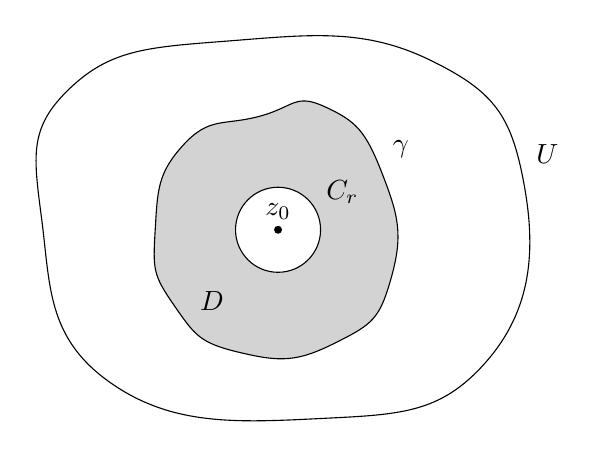
\begin{tikzpicture}[scale=1.2]
  % the open set U
  \draw plot[smooth cycle, tension=0.8] coordinates
    {(-2.5,0.2) (-2.2,1.6) (-0.5,2.1) (1.6,1.9) (2.6,0.6) (2.2,-1.3) (0.4,-1.9) (-1.8,-1.5)};
  \node at (2.85,0.9) {$U$};
  % region D between gamma and C_r
  \fill[gray, fill opacity=0.35, even odd rule]
    plot[smooth cycle, tension=0.9] coordinates
      {(-1.3,0.1) (-1.0,1.0) (-0.2,1.3) (0.5,1.4) (1.1,0.7) (1.2,-0.4) (0.6,-1.1) (-0.4,-1.2) (-1.1,-0.7)}
    (0,0.1) circle (0.45);
  \draw plot[smooth cycle, tension=0.9] coordinates
      {(-1.3,0.1) (-1.0,1.0) (-0.2,1.3) (0.5,1.4) (1.1,0.7) (1.2,-0.4) (0.6,-1.1) (-0.4,-1.2) (-1.1,-0.7)};
  \draw (0,0.1) circle (0.45);
  \fill (0,0.1) circle (1.2pt) node[above] {$z_0$};
  \node at (0.68,0.5) {$C_r$};
  \node at (1.3,0.95) {$\gamma$};
  \node at (-0.7,-0.65) {$D$};
\end{tikzpicture}
